\documentclass[a4,useAMS,usenatbib,usegraphicx,12pt]{article}
%External Packages and personalized macros
%=========================================================================
%		EXTERNAL PACKAGES
%=========================================================================
\usepackage[round]{natbib}
\usepackage[margin=3cm]{geometry}
\usepackage{hyperref}
\usepackage{times}
\usepackage{amsmath} 
\usepackage{amssymb}
\usepackage{graphicx}
\usepackage{array, xcolor, lipsum, bibentry}
\usepackage[nottoc, notlof, notlot]{tocbibind}

\definecolor{lightgray}{gray}{0.8}
\newcolumntype{L}{>{\raggedleft}p{0.14\textwidth}}
\newcolumntype{R}{p{0.8\textwidth}}
\newcommand\VRule{\color{lightgray}\vrule width 0.5pt}

\usepackage{booktabs}% http://ctan.org/pkg/booktabs
\newcommand{\tabitem}{~~\llap{\textbullet}~~}

%=========================================================================
%		INTERNAL MACROS
%=========================================================================
% To highlight comments 
\definecolor{red}{rgb}{1,0.0,0.0}
\newcommand{\red}{\color{red}}
\definecolor{darkgreen}{rgb}{0.0,0.5,0.0}
\newcommand{\SRK}[1]{\textcolor{darkgreen}{\bf SRK: \textit{#1}}}
\newcommand{\SRKED}[1]{\textcolor{darkgreen}{\bf #1}}

\newcommand{\LCDM}{$\Lambda$CDM~}
\newcommand{\beq}{\begin{eqnarray}}  
\newcommand{\eeq}{\end{eqnarray}}  
\newcommand{\zz}{$z\sim 3$} 
\newcommand{\apj}{ApJ}  
\newcommand{\apjs}{ApJS}  
\newcommand{\apjl}{ApJL}  
\newcommand{\aj}{AJ}  
\newcommand{\mnras}{MNRAS}  
\newcommand{\mnrassub}{MNRAS accepted}  
\newcommand{\aap}{A\&A}  
\newcommand{\aaps}{A\&AS}  
\newcommand{\araa}{ARA\&A}  
\newcommand{\nat}{Nature}  
\newcommand{\physrep}{PhR}
\newcommand{\pasp}{PASP}    
\newcommand{\pasj}{PASJ}    
\newcommand{\avg}[1]{\langle{#1}\rangle}  
\newcommand{\ly}{{\ifmmode{{\rm Ly}\alpha}\else{Ly$\alpha$}\fi}}
\newcommand{\hMpc}{{\ifmmode{h^{-1}{\rm Mpc}}\else{$h^{-1}$Mpc }\fi}}  
\newcommand{\hGpc}{{\ifmmode{h^{-1}{\rm Gpc}}\else{$h^{-1}$Gpc }\fi}}  
\newcommand{\hmpc}{{\ifmmode{h^{-1}{\rm Mpc}}\else{$h^{-1}$Mpc }\fi}}  
\newcommand{\hkpc}{{\ifmmode{h^{-1}{\rm kpc}}\else{$h^{-1}$kpc }\fi}}  
\newcommand{\hMsun}{{\ifmmode{h^{-1}{\rm {M_{\odot}}}}\else{$h^{-1}{\rm{M_{\odot}}}$}\fi}}  
\newcommand{\hmsun}{{\ifmmode{h^{-1}{\rm {M_{\odot}}}}\else{$h^{-1}{\rm{M_{\odot}}}$}\fi}}  
\newcommand{\Msun}{{\ifmmode{{\rm {M_{\odot}}}}\else{${\rm{M_{\odot}}}$}\fi}}  
\newcommand{\msun}{{\ifmmode{{\rm {M_{\odot}}}}\else{${\rm{M_{\odot}}}$}\fi}}  
\newcommand{\lya}{{Lyman$\alpha$~}}
\newcommand{\clara}{{\texttt{CLARA}}~}
\newcommand{\rand}{{\ifmmode{{\mathcal{R}}}\else{${\mathcal{R}}$ }\fi}}  


%MY COMMANDS #############################################################
\newcommand{\sub}[1]{\mbox{\scriptsize{#1}}}
\newcommand{\dtot}[2]{ \frac{ d #1 }{d #2} }
\newcommand{\dpar}[2]{ \frac{ \partial #1 }{\partial #2} }
\newcommand{\pr}[1]{ \left( #1 \right) }
\newcommand{\corc}[1]{ \left[ #1 \right] }
\newcommand{\lla}[1]{ \left\{ #1 \right\} }
\newcommand{\bds}[1]{\boldsymbol{ #1 }}
\newcommand{\oiint}{\displaystyle\bigcirc\!\!\!\!\!\!\!\!\int\!\!\!\!\!\int}
\newcommand{\mathsize}[2]{\mbox{\fontsize{#1}{#1}\selectfont $#2$}}
\newcommand{\eq}[2]{\begin{equation} \label{eq:#1} #2 \end{equation}}
\newcommand{\lth}{$\lambda_{th}$ }
%#########################################################################

\setlength\parindent{0pt}
 
\title{{\textbf{Research Proposal for a DAAD PhD scholarship}}\\ 
				The Gaseous Cosmic Web with AREPO\\ 
				\color{black}\rule{15cm}{0.5mm}}
\author{Sebastian Bustamante Jaramillo}
\date{}
  
\begin{document}
\maketitle
\begin{center}
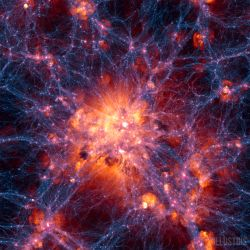
\includegraphics[trim = 0mm 3.5cm 0mm 3.0cm, clip, keepaspectratio=true,
width=0.7\textheight]{Presentation1.png}
\tiny{A projection of the cosmic web in the ILLUSTRIS simulation, that was made
with AREPO (http://www.illustris-project.org/)}
\end{center}
\tableofcontents
 
\newpage 

%============================================================================== 
\section{General Information}
\small
\subsection*{Information of the Applicant}
\begin{tabular}{L!{\VRule}R}
\bf Name		& Sebastian Bustamante Jaramillo\\
\bf Degree		& B.Sc. in Physics, Universidad de Antioquia (2013)\\
\bf Position	& Adjunct Professor, Universidad de Antioquia\\
\bf Birthday	& { 20$^{th}$ June, 1990}\\
\bf Nationality & Colombian\\
\bf ID			& C.C. 1128400433\\
\bf Address 1	& Avenida 21 \# 57 AA 65, Bello - Colombia (personal)\\
\bf Address 2	& Calle 67 \# 53 - 108, Off. 5-330, Medellin, Colombia (work)\\
\bf Phone		& +057 (4) 4820138\\
\bf Mobile		& +057 3108992409\\
\bf E-mail 1	& macsebas33 \textit{at} gmail.com (personal)\\
\bf E-mail 2	& sebastian.bustamante \textit{at} udea.edu.co (academic)\\
\end{tabular}

\vspace{10pt}

More detailed information of the applicant can be found here \url{http://goo.gl/BPZGzK}

\vspace{15pt}  

\subsection*{Information of the Project}
\begin{tabular}{L!{\VRule}R}
\bf Title		& \bf The Gaseous Cosmic Web with AREPO\\
\bf Field		& Cosmology, Astrophysics, Physical Sciences \\
\bf Advisor 1	& Professor Volker Springel. Heidelberg Institute for Theoretical Studies (HITS) 
\& University of Heidelberg, Germany \\
\bf Advisor 2	& Professor Jaime Forero-Romero, PhD. Universidad de los Andes, Colombia \\
\bf University	& University of Heidelberg, IMPRS PhD program \\
\bf Time Frame	& 3 years \\
\end{tabular}
\normalsize
%==============================================================================


%==============================================================================
\section{Abstract}
%==============================================================================


The cosmic web is one the most striking features of the Universe. It
has been widely tested by observations and studies through theory and
simulations. This web pattern has been studied in detail for the dark
matter distribution. Nevertheless, recent numerical work on
filamentary gas accretion demonstrated the need of hydrodynamical
simulations to understand galaxy evolution in the cosmic web. 
However, modelling gas dynamics is a complex task. Common hydro
solvers present accuracy problems that can bias the results of a
cosmic web study. However, recently a completely new simulation technique
was implemented in the \texttt{AREPO} code, which combines the
strength of previous schemes and overcomes their weaknesses. The main
aim of this PhD project is to perform a novel analysis of the
gaseous cosmic web using this new generation of hydrodynamical cosmological
simulations. 


\newpage

%==============================================================================
\section{Introduction}


The filamentary nature of the large-scale matter distribution (the so-called 
cosmic web) is one of the most striking features of the Universe \citep{Bond96}, 
The most recent generation of galaxy redshift surveys, such as the
\textit{two-degree-Field Galaxy  Redshift Survey} (2dFGRS, see
\citet{Colless03}) and the \textit{Sloan Digital  Sky Survey} (SDSS,
see \citet{Abazajian09}), have revealed the cosmic web with a great
level of detail. In addition, other observational probes like
the Ly-$\alpha$ forest in distant quasar spectra \citep{Rauch98, Cantalupo14} 
and weak gravitational lensing \citep{Massey07, Dietrich12} have also validated 
this picture.

\

On the theoretical side, Ya. B. Zeldovich \citep{Zeldovich70} provided
the founding insights into the physical mechanism driving the cosmic
web formation. Since then, our understanding of the structure and
dynamics of the cosmic web  has improved dramatically thanks to
powerful computational tools that became available. In  particular,
N-body simulations have played a key role in understanding the origin
and evolution of the Universe on its largest scales.

\

To obtain quantitative predictions from this paradigm it is necessary 
to specify the matter components of the Universe. In the current
cosmological paradigm there are two different types of matter. The
baryonic or luminous matter and the non-relativistic 
(i.e. cold) dark matter (DM). In our Universe the DM dominates the matter 
content as many different cosmological probes indicate \citep{Planck13XVI}. 

\

Accordingly, numerical research focuses on simulating dark matter
dominated universes, providing us with a detailed
understanding of the Universe on its largest scales. However, on small
(galactic) scales the effects of baryons become important. For instance,
recent simulations show that filamentary gas accretion in early stages
of galaxy evolution is a key physical process \citep{Dekel09}; there
is evidence that it plays a central role in the formation of discs
\citep{Dubois14}, determining the alignment of galaxies with respect
to the web \citep{Hahn10} and fueling high star formation rates
\citep{Dekel09}.  

\

Modelling baryons by incorporating gas dynamics into cosmological
simulations is a complex task. The main reason is that gas is
affected by a great variety of physical processes absent in dark
matter dynamics, mainly shocks and radiative cooling
\citep{Bond93}. Besides, there is the inherent complexity in
solving numerically the relevant equations. Traditionally, two
different hydro-solvers have been used by the astrophysical community
for this task. The first is a Lagrangian scheme on moving point masses
named \textit{Smoothed Particle Hydrodynamics} (\texttt{SPH}) 
\citep{Monaghan92} (for an implementation, see e.g. the \texttt{GADGET} 
code by \citet{Springel05}); the second is an Eulerian solver on a fixed 
mesh known as \textit{ Adaptive Mesh Refinement} (\texttt{AMR})
\citep{Berger89} (for an implementation,  see e.g. the \texttt{RAMSES}
code by \citet{Teyssier02}).  

\

The \texttt{SPH} scheme is easily implemented on a computer due to its 
Lagrangian character. Furthermore, as the physical systems evolves, the
mass particles naturally move into higher density regions providing a
self-adjusting spatial resolution. However, this scheme has been shown
to produce spurious suppression of fluid instabilities making it
unsuitable to model some of the dynamics accurately. 
On the other hand, \texttt{AMR} is more efficient 
for capturing shock dynamics. However, due to the conservative nature of the
hydrodynamical equations, the fixed mesh causes a lack of Galilean
invariance. Furthermore, the sampling of physical properties over the
grid introduces spurious vorticity to the fluid, making the scheme
unsuitable for studying turbulent flows. For a detailed  discussion
and comparison of \texttt{SPH} and \texttt{AMR} see \citet{Plewa01}).

\

Recently, a completely new approach to solve hydrodynamical problems was 
introduced by \citet{Springel10} and  implemented into the \texttt{AREPO}
code. It combines the strengths of  \texttt{AMR} and \texttt{SPH} but
overcomes many of their weaknesses. \texttt{AREPO} uses a moving mesh based
on a Voronoi tessellation defined over a set of particles that represents 
the fluid. The geometry of the mesh resembles very closely that 
of the point distribution retaining the auto-adaptivity inherent of
\texttt{SPH} and also keeping a grid to capture shocks like
\texttt{AMR} does. These features make \texttt{AREPO} highly 
efficient and accurate for simulating a wide range of hydrodynamical
problems, making it the best available approach for computing the
effects of the gaseous cosmic web in the Universe.

\
%here

Using a hydrodynamical simulation (\footnotesize{\texttt{HORIZON-AGN}}
\normalsize) computed through the \texttt{RAMSES} code, \citet{Dubois14} 
studied the alignment between the spin of galaxies and filaments above redshift
one. They found a redshift-dependent stellar mass threshold above which 
high-mass galaxies are misaligned with filaments, while low-mass galaxies are 
aligned. On the other hand, \citet{Hahn10} also studied this problem by mean of 
a \texttt{RAMSES} simulation, but finding a completely different result, 
high-mass galaxies are aligned while low-mass galaxies are misaligned with 
their embedding filaments. Some of these results may be affected by grid-alignment
effects of the disk, which occur in \texttt{AMR} codes such as \texttt{RAMSES}
but are absent in the moving-mesh code \texttt{AREPO}. Related to highly efficient 
star forming galaxies at high-redshifts, \citet{Dekel09} proposed a new scenario 
where the filamentary accretion of cold gas streams enhances the star formation 
rate. This is a very interesting alternative to the merger scenario, where star 
forming rates are propelled by violent collisions of galaxies. The new picture 
appears consistent with the observed properties of those galaxies, which exhibit
relatively intact rotating disks. All this shows the current interest in 
studying the impact of the gaseous cosmic web on galaxy evolution in the light 
of \texttt{AREPO} simulations, which make to possible to study 
deeper existing results and predict new ones.




%==============================================================================

\newpage
%==============================================================================
\section{Objectives}
%==============================================================================


\begin{itemize}

\item[\checkmark] Studying gaseous filamentary accretion of the cosmic web using 
\texttt{AREPO} simulations.

\item[\checkmark] Quantifying the impact of gaseous filamentary accretion on 
galaxy evolution.

\item[\checkmark] Deriving observable quantities from our theoretical studies.


\end{itemize}



%==============================================================================
\section{Methodology}
%==============================================================================


The proposed project is subject to a PhD study and will cover the following 
aspects:


\begin{itemize}

\item[\checkmark] \textit{First, an analysis and characterization of existing 
hydrodynamical simulations based on the \texttt{AREPO} code will be done.}

\end{itemize}


As this project will be entirely based on numerical results, an analysis and 
characterization of existing \texttt{AREPO} hydrodynamical simulations is one 
of the key steps. This includes a quantification of the dark matter and the 
gaseous cosmic web through two different web finding schemes (i.e. the T-web 
based on the tidal tensor \citep{Hahn07,Forero09}, and the V-web based on the 
velocity shear tensor \citep{Hoffman12}, schemes in which prof. Jaime 
Forero-Romero has a broad research experience); thus voids, walls, filaments 
and clusters will be identified. Then, a statistical analysis of the found 
structures will be carried out, i.e. volume and mass filling fractions at 
different redshifts, morphology, halo populations and filamentary accretion of 
gas.


In Heidelberg, the required computer facilities and access to existing 
simulations and the private \texttt{AREPO} code (of which Prof. Volker 
Springel is the main author) is granted. Moreover, the extensive research 
expertise of Prof. Springel in numerical cosmology is 
certainly another interest for pursuing this specific PhD project.


\begin{itemize}

\item[\checkmark] \textit{Second, detailed simulations of specific processes at
high redshifts will be computed.}

\end{itemize}


Once the gaseous cosmic web is analysed, we proceed by computing its impact on 
galaxy evolution, especially at high-redshifts due to the large amount of 
available observational constraints. This step involves computing new high 
resolution \texttt{AREPO} simulations in order to study specific processes 
like: star formation rate enhanced by filamentary gas accretion, angular 
momentum exchange between galaxies and the cosmic web, spin orientation of 
galaxies along filaments and walls.


\begin{itemize}

\item[\checkmark] \textit{Third, new observables will be derived based on the
results of the simulations. }

\end{itemize}


At this point, we will compare our theoretical results with available 
observational data of the cosmic web, specifically at high redshifts. This step 
will also involve deriving new observables based on our predictions.


%==============================================================================
\section{Current State}
%==============================================================================


At present the applicant has already the fundamental knowledge in Astrophysics and
Cosmology required for this investigation. This can be confirmed by his research
experience, including a paper (as co-author) published in the \textit{ApJL} in 
which the kinematics of the Local Group in a cosmological context was studied, 
another paper (as co-author) published in the \textit{ApJ} where the influence of 
thermal evolution on the magnetic habitability of rocky planets was studied,
and some participations in academic congresses. Furthermore, a Bachelor's thesis
\footnote{\scriptsize Further information and an electronic version of this 
thesis can be found here \url{https://github.com/sbustamante/Thesis}.} where the 
preferred place of simulated Local Group-like systems in the cosmic 
web was studied, also demonstrates the ability of the applicant for handling 
simulations and massive data, a skill that is necessary for carrying out this project.

\

Currently, the applicant is also involved in two research projects: first, a 
new method for finding voids in simulations based on the local fractional 
anisotropy is investigated. An ongoing publication (as first author) related to this is about 
to be submitted\footnote{\scriptsize Information of this paper can be found 
here \url{https://github.com/sbustamante/CosmicVoidsPaper}.}. The second project
involves a comparison of three simulation techniques, i.e. \texttt{SPH} vs 
\texttt{VPH} vs \texttt{AREPO}, with possible publishable results at the end of
the present year \footnote{\scriptsize Further information in  
\url{https://github.com/sbustamante/MethodsComparison}.}.


%==============================================================================
\section{Schedule}
%==============================================================================

\begin{table}[h]
\begin{flushleft}
\begin{center}
  \begin{tabular}{l  l} \hline\hline
	\centering\textbf{Year} & \textbf{Goals} \\ \hline
	%First year
	First  
	& \tabitem Identifying a set of existing \texttt{AREPO} simulations suitable 
	for our studies. \\
	& \tabitem Applying web finding schemes (T-web and V-web) to the simulations 
	for\\
	& \ \ \ \ quantifying structures in the gaseous cosmic web, i.e. voids, walls, 
	filaments\\
	& \ \ \ \ and clusters.\\
	& \tabitem Evaluating properties of found structures at different redshifts.\\
	\\
	%Second year	
	Second
	& \tabitem Studying by means of high resolution simulations the impact of the 
	gaseous\\
	& \ \ \ \ cosmic web on specific galaxy evolution processes.\\
	\\	
	%Third year	
	Third
	& \tabitem Comparing with available observational data of the cosmic web.\\
	& \tabitem Deriving new observable from our theoretical studies.\\ 
	
	\hline\hline
  \end{tabular}  
\end{center}
\end{flushleft}
\end{table}

\newpage
%==============================================================================
\bibliographystyle{latex/mn2e}
\renewcommand{\bibname}{8\ \ \ \ Bibliography}
\small
\bibliography{references.bib}
%==============================================================================



\end{document}
